\section{微分中值定理}

微分中值定理是微积分中的一个重要定理,它描述了函数在某一区间内的平均变化率与某一点处的瞬时变化率之间的关系. 

\subsection{四大基本定理}

\begin{lemma}[Fermat 引理]
    函数 $f(x)$ 在点 $x=\xi$ 的某邻域 $U(\xi)$ 内有定义,并且在 $\xi$ 处可导,如果对于任意的 $x\in U(\xi)$,
    都有 $f(x)\geqslant f(\xi)$ 或 $f(x)\geqslant f(\xi)$,那么 $f'(\xi)=0.$
\end{lemma}

\begin{theorem}[Rolle 定理]
    若 $f(x)$ 在 $[a,b]$ 上连续,在 $(a,b)$ 内可导,且 $f(b)=f(a)$,则 $\exists\xi\in(a,b)$,使得 $f'(\xi)=0.$
    \index{Rolle 定理}
\end{theorem}

\begin{example}
    设函数 $f(x)$ 在 $(0,+\infty)$ 内可导,且 $f(x)>0,~0<a<1$,证明存在 $\xi\in\left(a,\dfrac{1}{a}\right)$,
    使得 $$\dfrac{\xi f'(\xi)}{f(\xi)}=\dfrac{\xi^{-1}f'(\xi^{-1})}{f(\xi^{-1})}.$$
\end{example}
\begin{proof}[{\songti \textbf{证}}]
    将要证的等式化中的 $\xi$ 换成 $x$,并两边关于 $x$ 积分得
    $$\int\dfrac{f'(x)}{f(x)}\dd x=\int\dfrac{f'(x^{-1})}{f(x^{-1})}\dd x^{-1}\Rightarrow f(x)f(x^{-1})=C$$
    为此构造辅助函数 $$F(x)=f(x)f(x^{-1})$$
    于是 $f(x)\in C[0,1]\cap D(0,1)$,故由 Rolle 定理知,$\exists\xi\in(0,1)\text{,使得 }$
    $$F'(\xi)=f'(\xi)f(\xi^{-1})-\xi^{-2}f'(\xi^{-1})f(\xi)=0$$
    又 $\xi,f(\xi),f(\xi^{-1})\neq0$,故 $\dfrac{\xi f'(\xi)}{f(\xi)}=\dfrac{\xi^{-1}f'(\xi^{-1})}{f(\xi^{-1})}.$
\end{proof}

\begin{theorem}[Lagrange 定理]
    若 $f(x)$ 在 $[a,b]$ 上连续,在 $(a,b)$ 内可导,则 $\forall x_1,x_2\in[a,b],~\exists\xi\in(x_1,x_2)$,使得
    $$\dfrac{f(x_2)-f(x_1)}{x_2-x_1}=f'(\xi).$$
    \index{Lagrange 定理}
\end{theorem}

\begin{example}
    设 $f(x)$ 在 $[0,1]$ 上有连续的导数,证明 $$\lim_{n\to\infty}\sum_{k=1}^{n}\qty[f\qty(\dfrac{k}{n})-f\qty(\dfrac{2k-1}{2n})]=\dfrac{1}{2}\qty[f(1)-f(0)].$$
\end{example}
\begin{solution}
    由 Lagrange 中值定理知,$\exists\xi_k\in\qty(\dfrac{2k-1}{2n},\dfrac{k}{n})\text{,使 }f\qty(\dfrac{k}{n})-f\qty(\dfrac{2k-1}{2n})=\dfrac{f'(\xi_k)}{2n}$,
    于是
    \begin{flalign*}
        \lim_{n\to\infty}\sum_{k=1}^{n}\qty[f\qty(\dfrac{k}{n})-f\qty(\dfrac{2k-1}{2n})]=\dfrac{1}{2}\lim_{n\to\infty}\dfrac{1}{n}\sum_{k=1}^{n}f'(\xi_k)=\dfrac{1}{2}\int_{0}^{1}f(x)\dd x=\dfrac{1}{2}\qty[f(1)-f(0)].
    \end{flalign*}
\end{solution}

\begin{theorem}[Cauchy 定理]
    若 $F(x),G(x)$ 在 $[a,b]$ 上连续,在 $(a,b)$ 内可导,$G'(x)\neq0$,则 $\exists\xi\in(a,b)$,使得
    $$\dfrac{F(b)-F(a)}{G(b)-G(a)}=\dfrac{F'(\xi)}{G'(\xi)}.$$
    \index{Cauchy 定理}
\end{theorem}

\begin{example}
    设 $0<a<b$,证明至少存在一点 $\xi\in(a,b)$,使 $a\e ^b-b\e ^a=(1-\xi)\e ^{\xi}(a-b).$
\end{example}
\begin{proof}[{\songti \textbf{证}}]
    将要证的等式化为 $\dfrac{\dfrac{\e ^b}{b}-\dfrac{\e ^a}{a}}{\dfrac{1}{b}-\dfrac{1}{a}}=(1-\xi)\e ^\xi$,
    令 $f(x)=\dfrac{\e ^x}{x},~g(x)=\dfrac{1}{x}$,则 $f(x),g(x)$ 在 $[a,b]$ 上连续,在 $(a,b)$ 内可导,
    且 $\forall x\in(a,b),~g'(x)=-\dfrac{1}{x^2}<0$,故由 Cauchy 定理知,$\exists\xi\in(a,b)\text{,使得 }$
    $$\dfrac{f(b)-f(a)}{g(b)-g(a)}=\dfrac{f'(\xi)}{g'(\xi)}=(1-\xi)\e ^{\xi}$$
    化简得 $a\e ^b-b\e ^a=(1-\xi)\e ^{\xi}(a-b).$
\end{proof}

\begin{theorem}[Darboux 定理]
    设函数 $f(x)$ 在 $[a,b]$ 上处处可导 (端点指单侧导数),$f'(a)<f'(b)$ 或 $f'(a)>f'(b)$,
    则 $\forall\mu:f'(a)<\mu <f'(b)$,或 $f'(a)>\mu>f'(b)$,$\exists\xi\in(a,b)$,使得 $f'(\xi)=\mu.$
    \index{Darboux 定理}
\end{theorem}

\subsection{单中值问题}

\subsubsection{辅助函数的构造}

常用的辅助函数构造,本质为解微分方程.
\setcounter{magicrownumbers}{0}
\begin{table}[H]
    \caption{}
    \centering
    \resizebox{.99\textwidth}{!}{
        \begin{tabular}{l l l l}
            原函数                                   & 辅助函数                        & 原函数                                        & 辅助函数                              \\
            (\rownumber{}) $\xi f'(\xi)+nf(\xi)=0$    & $F(x)=x^nf(x)$                  & (\rownumber{}) $\xi f'(\xi)-nf(\xi)=0$         & $F(x)=x^{-n}f(x)$                     \\
            (\rownumber{}) $f'(\xi)+\lambda f(\xi)=0$ & $F(x)=\e^{\lambda x}f(x)$       & (\rownumber{}) $\alpha f'(\xi)+\beta f(\xi)=0$ & $F(x)=\e^{\frac{\beta}{\alpha}x}f(x)$ \\
            \midrule
            (\rownumber{}) $f'(\xi)+g'(\xi)f(\xi)=0$  & $F(x)=\e^{g(x)}f(x)$            & (\rownumber{}) $f'(\xi)+g(\xi)f(\xi)=0$        & $F(x)=\e^{\int g(x)}f(x)$             \\
            (\rownumber{}) $f'(x)-\lambda (f(x)-x)=1$ & $F(x)=(f(x)-x)\e ^{-\lambda x}$ & (\rownumber{}) $f'(x)-\alpha (f(x)-f(a))=0$    & $F(x)=(f(x)-f(a))\e ^{-\alpha x}$     \\
            \midrule
            (\rownumber{}) $f''(x)+f(x)=0$            & $F(x)=f^2(x)+\qty[f'(x)]^2$     & (\rownumber{}) $f''(x)-f(x)=0$                 & $F(x)=\e ^x(f'(x)-f(x))$              \\
        \end{tabular}}
    \label{fuzuhansgzao}
\end{table}
\begin{proof}[{\songti \textbf{证}}]
    关于如何解微分方程可参考阅读第八章.
    \begin{enumerate}[label=(\arabic{*})]
        \item 将原函数改写为 $\displaystyle x\dv{y}{x}+ny=0$,该方程是变量分离方程,即
              $$\dfrac{\dd x}{x}=-\dfrac{\dd y}{ny}\Rightarrow \int\dfrac{\dd x}{x}=-\dfrac{1}{n}\int\dfrac{\dd y}{y}\Rightarrow\ln x^n+\ln y=C\Rightarrow x^ny=C$$
              将 $C$ 改写为 $F(x)$,即得辅助函数 $F(x)=x^nf(x)$.
        \item 同 (1) 易得 $\dfrac{y}{x^n}=C$,因此辅助函数为 $F(x)=\dfrac{f(x)}{x^n}.$
        \item 将原函数改写为 $y'+\lambda y=0$,有通解 $y=C\e^{-\lambda x}$,即 $C=y\e^{\lambda x}$,将 $C$ 改写为 $F(x)$,即得辅助函数 $F(x)=\e^{\lambda x}f(x).$
        \item 同 (2) 得通解 $y=C\e^{-\frac{\beta}{\alpha}x}$,即 $C=y\e^{\frac{\beta}{\alpha}x}$,因此有辅助函数 $F(x)=\e^{\frac{\beta}{\alpha}x}f(x).$
        \item 将原函数改写为 $y'+g'(x)y=0$,该方程为一阶常系数线性微分方程,有通解 $y=C\e^{-\int g'(x)\dd x}$,即 $C=y\e^{g(x)}$,因此有辅助函数 $F(x)=\e^{g(x)}f(x).$
        \item 同 (5) 易得辅助函数为 $F(x)=\e^{\int g(x)}f(x).$
        \item 将原函数改写为 $y'-\lambda(y-x)=1\Rightarrow y'-\lambda y=1-\lambda x$,该方程为一阶常系数线性微分方程,有通解为
              $$y=\e^{\int\lambda\dd x}\qty[\int(1-\lambda x)\e^{-\int\lambda\dd  x}\dd x+C]=x+C\e^{\lambda x}$$
              即 $C=(y-x)\e^{-\lambda x}$,因此辅助函数为 $F(x)=(f(x)-x)\e^{-\lambda x}.$
        \item 同 (7) 原函数为 $y'-\alpha f(x)=-\alpha f(a)$,有通解为
              $$y=\e^{\alpha\int\dd x}\qty[-\alpha f(a)\int\e^{-\alpha \int\dd x}\dd x+C]=f(a)+C\e^{\alpha x}$$
              即 $C=(y-f(a))\e^{-\alpha x}$,因此辅助函数为 $F(x)=(f(x)-f(a))\e^{-\alpha x}.$
        \item 将原函数改写为 $y''+y=0$,等式两边同时乘以 $2y'$,有 $2y'y''+2yy'=0\Rightarrow \qty[(y')^2+y^2]'=C$,因此辅助函数为 $F(x)=f^2(x)+\qty[f'(x)]^2.$
        \item 将原函数改写为 $y''-y=0$ 并令 $\displaystyle \mathrm{D}=\dv{x}$,于是有 $\qty(\mathrm{D}^2-1)y=(\mathrm{D}+1)(\mathrm{D}-1)y=0$,令 $(\mathrm{D}-1)y=z$,则
              $$\dv{z}{x}+z=0\Rightarrow z=C\e^{-x}\Rightarrow C=(\mathrm{D}-1)y\e^{x}$$
              将 $C$ 改写为 $F(x)$,即得辅助函数 $F(x)=\e^{x}(f'(x)-f(x)).$
    \end{enumerate}
\end{proof}

\begin{example}
    设函数 $f(x),g(x)\in C[a,b]\cap D(a,b)$,且 $f(a)=f(b)=0$,证明至少存在一点 $\xi\in(a,b)$,
    使得 $f'(\xi)+f(\xi)g'(\xi)=0.$
\end{example}
\begin{proof}[{\songti \textbf{证}}]
    将要证的等式化中的 $\xi$ 换成 $x$,有 $f'(x)+f(x)g'(x)=0$,化为 $\dfrac{f'(x)}{f(x)}-g'(x)$,
    然后两边关于 $x$ 积分,得 $$\ln|f(x)|=-g(x)+C\Rightarrow f(x)=C\e ^{-g(x)}\Rightarrow f(x)\e ^{g(x)}=C$$
    为此构造辅助函数
    $$F(x)=f(x)\e ^{g(x)}$$
    则 $F(x)$ 在 $[a,b]$ 上连续,在 $(a,b)$ 内可导,故由 Rolle 定理知,$\exists\xi\in(a,b)\text{,使得 }$
    $$F'(\xi)=(f'(\xi)+f(\xi)\cdot g'(\xi))\e ^{g(\xi)}=0$$
    而 $\e ^{g(x)}>0$,故 $f'(\xi)+f(\xi)\cdot g'(\xi)=0.$
\end{proof}

\begin{example}
    设函数 $f(x)\in C[0,1]\cap D(0,1)$,$f(0)=0$,且 $\forall x\in(0,1)$,都有 $f(x)\neq0$,证明至少存在一点 $\xi\in(0,1)$,使得
    $\dfrac{nf'(\xi)  }{f(\xi)  }=\dfrac{f'(1-\xi)  }{f(1-\xi)  }$,其中 $n$ 为自然数.
\end{example}
\begin{proof}[{\songti \textbf{证}}]
    将要证的等式化中的 $\xi$ 换成 $x$,并两边关于 $x$ 积分得
    $$n\ln \left| f(x)  \right| =-\ln \left| f\left( 1-x\right) \right| +C\Rightarrow f^{n}(x)  \cdot f\left( 1-x\right) =C$$
    为此构造辅助函数 $$F(x)=f^{n}(x)  \cdot f\left( 1-x\right)$$
    那么 $f(x)\in C[0,1]\cap D(0,1)$,$F(0)=F(1)$,故有 Rolle 定理知,
    $$\exists\xi\in(0,1)\text{,使得 }F'(\xi)=nf^{n-1}(\xi) f'(\xi) f(1-\xi)  -f^{n}(\xi)  f'(1-\xi)  =0$$
    又 $f(\xi),f(1-\xi)\neq0$,故有 $nf'(\xi)  f(1-\xi)  -f(\xi)  f'(1-\xi)  =0$,
    即 $\dfrac{nf'(\xi)  }{f(\xi)  }=\dfrac{f'(1-\xi)  }{f(1-\xi)  }.$
\end{proof}
\begin{inference}
    设函数 $f(x)\in C[0,1]\cap D(0,1)$,$f(0)=0$,且 $\forall x\in(0,1)$,都有 $f(x)\neq0$,则由
    至少存在一点 $\xi\in(0,1)$,使得
    $$\dfrac{mf'(\xi)  }{f(\xi)  }=\dfrac{nf'(1-\xi)  }{f(1-\xi)  }$$
    其中 $m,n$ 为自然数.
\end{inference}

\begin{example}
    设 $f(x)\in C\qty[0,\dfrac{\pi}{2}]\cap D\qty(0,\dfrac{\pi}{2}),~f(0)=f\qty(\dfrac{\pi}{2})=\dfrac{1}{2}$,证明: $\exists\xi\in\qty(0,\dfrac{\pi}{2})$,使得 $f'(\xi)+f(\xi)=\cos\xi.$
\end{example}
\begin{proof}[{\songti \textbf{证}}]
    构造辅助函数\footnote{
        解一阶线性微分方程
        \begin{flalign*}
            y=\e^{-\int\dd x}\qty[\int\cos x\cdot\e^{\int\dd x}\dd x+C]=\e^{-x}\qty[\int\cos x\e^{x}\dd x+C]=\dfrac{1}{2}(\sin x+\cos x)+C\e^{-x}
        \end{flalign*}
        其中 $\displaystyle\int\cos x\e^{x}\dd x=\dfrac{\mqty|\qty(\e^{x})'&(\cos x)'\\\e^{x}&\cos x|}{2}+C=\dfrac{1}{2}(\sin x+\cos x)+C.$
    } $F(x)=\e^xf(x)-\dfrac{\e^x}{2}\cdot(\sin x+\cos x)$,则 $$F(0)=F\qty(\dfrac{\pi}{2})=0$$
    由 Rolle 定理知,$\exists\xi\in\qty(0,\dfrac{\pi}{2})$,使得 $$F'(\xi)=\e^\xi\qty[f'(\xi)+f(\xi)-\cos\xi]=0$$
    又 $\e^\xi>0$,因此 $f'(\xi)+f(\xi)=\cos\xi.$
\end{proof}

\begin{example}[第十届 “景润杯”]
    设 $f(x),g(x)\in C[a,b]\cap D(a,b)$,且满足 $$2b>3a,~a+b>0,~f(a)=0,~f\qty(\dfrac{2a+2b}{5})+f\qty(\dfrac{3a+3b}{5})=0$$
    证明存在一点 $\xi\in(a,b)$,使得 $f'(\xi)+f(\xi)g'(\xi)=0.$
\end{example}
\begin{proof}[{\songti \textbf{证}}]
    令 $h(x)=f(x)\e ^{g(x)}$,
    由题意可得 $\dfrac{2a+3b}{5},\dfrac{3a+3b}{5}\in(a,b)$,由 $f\qty(\dfrac{2a+2b}{5})+f\qty(\dfrac{3a+3b}{5})=0$,可得
    $$f\qty(\dfrac{2a+2b}{5})\cdot f\qty(\dfrac{3a+3b}{5})<0\text{ 或 }f\qty(\dfrac{2a+2b}{5})=f\qty(\dfrac{3a+3b}{5})=0$$
    若 $f\qty(\dfrac{2a+2b}{5})\cdot f\qty(\dfrac{3a+3b}{5})<0$,则由零点定理知,$\exists\eta\in\qty(\dfrac{2a+2b}{5},\dfrac{3a+3b}{5})$,使得 $f(\eta)=0$;
    若 $f\qty(\dfrac{2a+2b}{5})=f\qty(\dfrac{3a+3b}{5})=0$,则取 $\eta=\dfrac{2a+2b}{5}$,那么 $f(\eta)=0$,
    显然 $[a,\eta]\subset [a,b]$,且 $h(x)$ 在 $[a,\eta]$ 上满足 Rolle 定理的条件,则 $\exists\xi\in(a,\eta)\subset(a,b)\text{,使得 }h'(\xi)=0$,
    而 $h'(\xi)=\e ^{g(\xi)}\qty[f'(\xi)+f(\xi)g'(\xi)]=0$,因 $\e ^{g(\xi)}\neq0$,故 $f'(\xi)+f(\xi)g'(\xi)=0.$
\end{proof}

\subsubsection{常数 $k$ 值法}
一般用于端点函数值不确定的情况下,即题目中没有说明 $f(a)$ 与 $f(b)$ 的值,此时令带有中值的函数 $\varphi(\xi)=k$,再将待证式中的一端点 $b$ (或者 $a$) 改写为 $x$ 即得辅助函数.

\begin{example}
    设 $0<a<b$,函数 $f(x)\in C[a,b]\cap D(a,b)$,证明至少存在一点 $\xi\in(a,b)$,使得 $$f(b)-f(a)=\xi f'(\xi)\ln\dfrac{b}{a}.$$
\end{example}
\begin{proof}[{\songti \textbf{证法一}}]
    将要证式化为 $\dfrac{f(b)-f(a)}{\xi}=f'(\xi)\ln\dfrac{b}{a}$,即需证明
    $\left[ \left( f(b)  -f(a)  \right) \ln x\right] _{x=\xi }^{'}=\left[ f(x)  \ln \dfrac{b}{a}\right] _{x=\xi }^{'}$,
    为此,作辅助函数 $$F(x)  =\left( f(b)  -f(a)  \right) \ln x-f(x)  \ln \dfrac{b}{a}$$
    则 $F(x)$ 在 $[a,b]$ 上连续,在 $(a,b)$ 内可导,且 $F(b)=F(a)$,故由 Rolle 定理知,$\exists\xi\in(a,b)\text{,使得 }$
    $$F'(\xi)=(f(b)-f(a))\dfrac{1}{\xi}-f'(\xi)\ln\dfrac{b}{a}=0$$
    即 $f(b)-f(a)=\xi f'(\xi)\ln\dfrac{b}{a}.$
\end{proof}
\begin{proof}[{\songti \textbf{证法二}}]
    将要证式化为 $\dfrac{f(b)  -f(a)  }{\ln b-\ln a}=\xi f'(\xi)  $,
    令 $\dfrac{f(b)  -f(a)  }{\ln b-\ln a}=k$,则 $f(b)-k\ln b=f(a)-k\ln a$,此时只需证 $k=\xi f'(\xi)$,
    为此,作辅助函数 $$F(x)=f(x)-k\ln x$$ 则 $F(x)$ 在 $[a,b]$ 上连续,在 $(a,b)$ 内可导,且 $F(b)=F(a)$,故由 Rolle 定理知,$\exists\xi\in(a,b)\text{,使得 }$
    $$F'(\xi)=f'(\xi)-\dfrac{k}{\xi}=0$$
    即得 $k=\xi f'(\xi)$,从而得 $f(b)-f(a)=\xi f'(\xi)\ln\dfrac{b}{a}.$
\end{proof}
\begin{proof}[{\songti \textbf{证法三}}]
    要证 $f(b)-f(a)=\xi f'(\xi)\ln\dfrac{b}{a}$,只需设 $k$ 为使等式 $f(b)-f(a)=k\cdot\ln\dfrac{b}{a}$ 成立的待定常数,再证明 $k=\xi f'(\xi)$ 即可,
    为此,将等式中的 $b$ 改写为 $x$,并移项,构造辅助函数
    $$F(x)=f(x)-f(a)-k\ln\dfrac{x}{a}$$
    则 $F(x)$ 在 $[a,b]$ 上连续,在 $(a,b)$ 内可导,且 $F(b)=0=F(a)$,于是由 Rolle 定理知,$\exists\xi\in(a,b)\text{,使得 }$
    $$F'(\xi)=f'(\xi)-\dfrac{k}{\xi}=0$$
    即得 $k=\xi f'(\xi)$,从而得证.
\end{proof}
\begin{proof}[{\songti \textbf{证法四}}]
    将要证的等式化为 $\dfrac{f(b)-f(a)}{\ln b-\ln a}=\dfrac{f'(\xi)}{\dfrac{1}{\xi}}$,易见,设 $g(x)=\ln x$,则
    $f(x),g(x)$ 在 $[a,b]$ 上连续,在 $(a,b)$ 内可导,且 $\forall x\in(a,b),g'(x)=\dfrac{1}{x}\neq0$,故由 Cauchy 中值定理知,$\exists\xi\in(a,b)\text{,使得 }$
    $$\dfrac{f(b)-f(a)}{g(b)-g(a)}=\dfrac{f'(\xi)}{g'(\xi)}$$
    即 $\dfrac{f(b)-f(a)}{\ln b-\ln a}=\dfrac{f'(\xi)}{g'(\xi)}$,化简得 $f(b)-f(a)=\xi f'(\xi)\ln\dfrac{b}{a}.$
\end{proof}
证法二 又称为第一类常数 $k$ 值法,主要适用于常数部分可以分离的微积分中值等式证明题; 证法三则称为第二类常数 $k$ 值法,适用面更广.
\begin{inference}
    设函数 $f(x),g(x)\in C[a,b]\cap D(a,b)$,且 $g'(x)\neq0$,又 $g(x)>0,a\leqslant x\leqslant b$,则存在一点 $\xi\in(a,b)$,使得\label{gfbfagf}
    $$g'(\xi)  \left[ f(b)  -f(a)  \right] =g(\xi)  f'(\xi)  \ln \dfrac{g(b)  }{g(a)  }.$$
\end{inference}
\begin{proof}[{\songti \textbf{证}}]
    因为 $f(x),g(x)$ 皆在 $[a,b]$ 上连续,在 $(a,b)$ 内可导,且 $g'(x)\neq0$,又 $g(x)>0,a\leqslant x\leqslant b$,
    所以由 Cauchy 定理知 $\exists\xi\in(a,b)$,使得
    $$\dfrac{\ln g(b)-\ln g(a)}{f(b)-f(a)}=\dfrac{g'(\xi)}{g(\xi)f'(\xi)}$$
    整理即得待证式.
\end{proof}

\begin{example}
    设 $0<a<b$,函数 $f(x)\in C[a,b]\cap D(a,b)$,证明 $\exists\xi\in(a,b)$,使得
    $$2\xi[f(b)-f(a)]=(b^2-a^2)f'(\xi).$$
\end{example}
\begin{proof}[{\songti \textbf{证法一}}]
    要证 $2\xi[f(b)-f(a)]=(b^2-a^2)f'(\xi)$,只需证
    $$\left[x^2\cdot(f(b)-f(a))\right]'_{x=\xi}=\left[(b^2-a^2)f(x)\right]'_{x=\xi}$$
    为此,构造辅助函数 $F(x)=x^2\cdot(f(b)-f(a))-(b^2-a^2)f(x)$,那么 $F(x)$ 在 $[a,b]$ 上连续,在 $(a,b)$ 内可导,
    且 $F(a)=F(b)$,故由 Rolle 定理知,$\exists\xi\in(a,b)\text{,使得 }$
    $$F'(\xi)=2\xi(f(b)-f(a))-(b^2-a^2)f'(\xi)=0$$
    即 $2\xi[f(b)-f(a)]=(b^2-a^2)f'(\xi).$
\end{proof}
\begin{proof}[{\songti \textbf{证法二}}]
    将要证的等式化为 $2\xi\dfrac{f(b)-f(a)}{b^2-a^2}=f'(\xi)$,令 $\dfrac{f(b)-f(a)}{b^2-a^2}=k$,则 $f(b)-kb^2=f(a)-ka^2$,
    为此,构造辅助函数 $$F(x)=f(x)-kx^2$$
    则 $F(x)$ 在 $[a,b]$ 上连续,在 $(a,b)$ 内可导,且 $F(a)=F(b)$,故由 Rolle 定理知,$\exists\xi\in(a,b)\text{,使得 }$
    $$F'(\xi)=f'(\xi)-2k\xi =0$$
    即 $f'(\xi)=2k\xi$,因而在 $\dfrac{f(b)-f(a)}{b^2-a^2}=k$ 的两边同时乘以 $2\xi (b^2-a^2)$,即得待证等式.
\end{proof}
\begin{proof}[{\songti \textbf{证法三}}]
    将要证的等式化为 $f(b)-f(a)=\dfrac{f'(\xi)}{2\xi}(b^2-a^2)$,设 $k$ 为使 $f(b)-f(a)=k(b^2-a^2)$ 成立的实常数,
    则只需证 $k=\dfrac{f'(\xi)}{2\xi}$,为此构造辅助函数:
    $$F(x)=f(x)-f(a)-k(x^2-a^2)$$
    则 $F(x)$ 在 $[a,b]$ 上连续,在 $(a,b)$ 内可导,且 $F(a)=F(b)$,故由 Rolle 定理知,$\exists\xi\in(a,b)\text{,使得 }$
    $$F'(\xi)=f'(\xi)-2k\xi=0$$
    即得 $f'(\xi)=2k\xi$,又 $0<a<b,~\xi\in(a,b)$,所以 $\xi>0$,于是 $k=\dfrac{f'(\xi)}{2\xi}$,从而得证.
\end{proof}
\begin{proof}[{\songti \textbf{证法四}}]
    将要证的等式化为 $\dfrac{f(b)-f(a)}{b^2-a^2}$,令 $g(x)=x^2$,则 $f(x),g(x)$ 在 $[a,b]$ 上连续,在 $(a,b)$ 内可导,且
    $\forall x\in(a,b),~g'(x)=2x>0$,故由 Cauchy 定理知,$\exists\xi\in(a,b)\text{,使得 }$
    $$\dfrac{f(b)-f(a)}{b^2-a^2}=\dfrac{f'(\xi)}{g'(\xi)}$$
    化简得 $2\xi[f(b)-f(a)]=(b^2-a^2)f'(\xi).$
\end{proof}
\begin{inference}
    一般地,设函数 $f(x),g(x)\in C[a,b]\cap D(a,b)$,则 $\exists\xi\in(a,b)\text{,使得 }$
    $$g'(\xi)(f(b)-f(a))=(g(b)-g(a))f'(\xi).$$
\end{inference}
\begin{proof}[{\songti \textbf{证}}]
    由 Cauchy 定理易证.
\end{proof}

\begin{example}
    设函数 $f(x)\in C[a,b]\cap D(a,b)$,证明 $\exists\xi\in(a,b)$,
    使得 $\dfrac{f(\xi)-f(a)}{b-\xi}=f'(\xi).$
\end{example}
\begin{proof}[{\songti \textbf{证法一}}]
    将要证的等式化为 $f(\xi)  +\xi f'(\xi)  -f(a)  -bf'(\xi)  =0$,即只需证
    $\left[ xf(x)  -f(a)  x-bf(x)  \right] _{x=\xi }'$,为此构造辅助函数
    $$F(x)  =xf(x)  -f(a)  x-bf(x)  $$
    则 $F(x)$ 在 $[a,b]$ 上连续,在 $(a,b)$ 内可导,且 $F(a)=-bf(a)=F(b)$,故由 Rolle 定理知,$\exists\xi\in(a,b)\text{,使得 }$
    $$F'(\xi)=f(\xi)+\xi f'(\xi)-f(a)-bf'(\xi)=0$$
    化简即得 $\dfrac{f(\xi)-f(a)}{b-\xi}=f'(\xi).$
\end{proof}
\begin{proof}[{\songti \textbf{证法二}}]
    将要证的等式化中的 $\xi$ 化为 $x$,有 $\dfrac{f(x)-f(a)}{b-x}=f'(x)  \Rightarrow\dfrac{1}{b-x}=\dfrac{[f(x)-f(a)]'}{f(x)-f(a)}$,两边关于 $x$ 积分得 $$-\ln(b-x)=\ln|f(x)-f(a)|+\ln C$$
    即 $(b-x)(f(x)-f(a))\equiv C.$,为此构造辅助函数
    $$F(x)=(b-x)(f(x)-f(a))$$
    则 $F(x)$ 在 $[a,b]$ 上连续,在 $(a,b)$ 内可导,且 $F(a)=0=F(b)$,故由 Rolle 定理知,$\exists\xi\in(a,b)\text{,使得 }$
    $$F'(\xi)=bf'(\xi)-f(\xi)-\xi f'(\xi)+f(a)=0$$
    化简即得 $\dfrac{f(\xi)-f(a)}{b-\xi}=f'(\xi).$
\end{proof}
\begin{proof}[{\songti \textbf{证法三}}]
    将要证的等式化为 $(b-\xi)f'(\xi)-f(\xi)=-f(a)=-\dfrac{(b-a)f(a)}{b-a}$,为此构造辅助函数
    $$F(x)=(b-x)f(x)$$ 则 $F(x)$ 在 $[a,b]$ 上连续,在 $(a,b)$ 内可导,
    故由 Lagrange 中值定理知,$\exists\xi\in(a,b)\text{,使得 }$
    $$\dfrac{F(b)-F(a)}{b-a}=F'(\xi)=-f(\xi)+(b-\xi)f'(\xi)$$
    即得 $f'(\xi)=\dfrac{f(\xi)-f(a)}{b-\xi}.$
\end{proof}
\begin{proof}[{\songti \textbf{证法四}}]
    将要证的等式化为 $f(\xi)-f(a)+\xi f'(\xi)=bf'(\xi)$,即只需证 $$\dfrac{1}{b}=\dfrac{f'(\xi)}{f(\xi)-f(a)+\xi f'(\xi)}$$
    而 $f(\xi)-f(a)+x\xi f'(\xi)=\left[xf(x)-f(a)x\right]'_{x=\xi}$,为此构造辅助函数
    $$F(x)=x(f(x)-f(a))$$
    则 $f(x),F(x)$ 在 $[a,b]$ 满足 Cauchy 中值定理的条件,于是 $\exists\xi\in(a,b)\text{,使得 }$
    $$\dfrac{f(b)-f(a)}{F(b)-F(a)}=\dfrac{f'(\xi)}{F'(\xi)}$$
    化简即得 $\dfrac{f(\xi)-f(a)}{b-\xi}=f'(\xi).$
\end{proof}
\begin{inference}
    设函数 $f(x),g(x)\in C[0,1]\cap D(0,1)$,且对任意的 $x\in(a,b)$,有 $g'(x)\neq0$,
    则至少存在一点 $\xi\in(a,b)$,使得 $$\dfrac{f(\xi)-f(a)}{g(b)-g(\xi)}=\dfrac{f'(\xi)}{g'(\xi)}.$$
\end{inference}
\begin{proof}[{\songti \textbf{证}}]
    要证 $\dfrac{f(\xi)-f(a)}{g(b)-g(\xi)}=\dfrac{f'(\xi)}{g'(\xi)}$,只需证 $(g(\xi)-g(b))f'(\xi)+(f(\xi)-f(a))g'(\xi)=0$,
    即证 $$(g(x)f(x)-g(b)f(x)-f(a)g(x))'_{x=\xi}=0$$
    为此构造辅助函数 $F(x)=(f(x)-f(a))(g(x)-g(b))$ 则 $F(x)$ 在 $[a,b]$ 上连续,在 $(a,b)$ 内可导,
    $F(a)=F(b)$ 故由 Rolle 定理知,$\exists\xi\in(a,b)\text{,使得 }$
    $$F'(\xi)=f'(\xi)(g(\xi)-g(b))g'(\xi)(f(\xi)-f(a))=0$$
    即得 $\dfrac{f(\xi)-f(a)}{g(b)-g(\xi)}=\dfrac{f'(\xi)}{g'(\xi)}.$
\end{proof}

\subsection{双中值问题}

证明含有两个中值 (可相等) 微分等式的常见方法有:
\begin{enumerate}[label=(\arabic{*})]
    \item 使用两次 Lagrange 中值定理;
    \item 使用两次 Cauchy 中值定理;
    \item 使用两次 Taylor 中值定理;
    \item 使用 Rolle 定理、Lagrange 中值定理及 Cauchy 中值定理中的任两个定理各一次.
\end{enumerate}
对于含有三个中值微分等式的证明题,其证明方法可以类似地推广得到.
如果两个中值不相等,那么可对\textbf{区间进行划分},在各自的子区间运用中值定理.

\subsubsection{区间无需划分}

\begin{example}
    设函数 $f(x)\in C[0,1]\cap D(0,1)$,且 $f(a)=f(b)=1$,证明存在 $\xi,\eta\in(a,b)$,使得 $\e ^{\eta-\xi}[f(\eta)-f'(\eta)]=1.$
\end{example}
\begin{proof}[{\songti \textbf{证法一}}]
    将要证明的等式中含 $\xi$ 和 $\eta$ 的项分别放到等式的两侧,化为
    $$\e ^{\eta }\left[ f(\eta)  +f'(\eta)  \right] =\e ^{\xi }$$
    即只需证 $[\e f(x)]'_{x=\eta}=\left(\e ^x\right)'_{x=\xi}$,而由 Lagrange 中值定理知,
    $$\dfrac{\e ^b-\e ^a}{b-a}=\left(\e ^x\right)'_{x=\xi},~\dfrac{\e ^bf(b)-\e ^af(a)}{b-a}=[\e f(x)]'_{x=\eta}$$
    且 $f(a)=f(b)=1$ 知 $\dfrac{\e ^b-\e ^a}{b-a}=\dfrac{\e ^bf(b)-\e ^af(a)}{b-a}$,故可令
    $$F(x)=\e ^xf(x),~G(x)=\e ^x$$
    则 $F(x),G(x)$ 在 $[a,b]$ 上连续,在 $(a,b)$ 内可导,于是分别对 $F(x)$ 和 $G(x)$ 用 Lagrange 中值定理知
    $\exists\xi,\eta\in(a,b)\text{,使得 }$
    $$\dfrac{\e ^b-\e ^a}{b-a}=\left(\e ^x\right)'_{x=\xi}=\e ^\xi,~\dfrac{\e ^bf(b)-\e ^af(a)}{b-a}=[\e f(x)]'_{x=\eta}=\e ^\eta[f(\eta)+f'(\eta)]$$
    又 $f(a)=f(b)=1$,从而得 $\e ^{\eta }\left[ f(\eta)  +f'(\eta)  \right] =\e ^{\xi }$,即 $\e ^{\eta-\xi}[f(\eta)-f'(\eta)]=1.$
\end{proof}
\begin{proof}[{\songti \textbf{证法二}}]
    要证 $\e ^{\eta-\xi}[f(\eta)-f'(\eta)]=1$,即要证 $\e ^{\eta-\xi}[f(\eta)-f'(\eta)]-1=0$,将 $\eta$ 改写为 $x$ 后,
    只需证 $\left[\e ^{x-\xi}\cdot f(x)-x\right]'_{x=\eta}=0$,为此构造辅助函数
    $$F(x)=\e ^{x-\xi}\cdot f(x)-x$$
    即证 $F(x)$ 满足 Rolle 定理,而这需要证明 $F(b)=F(a)$,即 $\e ^{b-\xi}-\e ^{a-\xi}=b-a$,
    再令 $G(x)=\e ^x$,则 $G(x)$ 在 $[a,b]$ 上连续,在 $(a,b)$ 内可导,由 Lagrange 中值定理知,$\exists\xi\in(a,b)\text{,使得 }$
    $$G(b)-G(a)=G'(\xi)(b-a)$$
    从而得 $F(a)=F(b)$,故由 Rolle 定理知,$\exists\eta\in(a,b)\text{,使得 }F'(\eta)=0$,
    即 $\e ^{\eta-\xi}[f(\eta)-f'(\eta)]=1.$
\end{proof}

\begin{example}
    设 $f(x)\in C[0,1]\cap D(0,1)$,证明: $\exists\xi,\eta\in(0,1)$,使得 $$\e^{\eta-1}\qty[f(\xi)+\xi f'(\xi)]=\eta f'(\eta)+f(\eta)-\eta f(\eta).$$
\end{example}
\begin{proof}[{\songti \textbf{证}}]
    对 $xf(x)$ 在 $[0,1]$ 上使用 Lagrange 中值定理,有
    $$\dfrac{1\cdot f(1)-0}{1-0}=f(\xi)+\xi f'(\xi)=1,~\xi\in(0,1)$$
    对 $x\e^{-x}f(x)$ 在 $[0,1]$ 上使用 Lagrange 中值定理,有
    $$\dfrac{\e^{-1}f(1)-0}{1-0}=\e^{-\eta}\qty[\eta f'(\eta)+f(\eta)-\eta f(\eta)]=\e^{-1}f(\eta),~\eta\in(0,1)$$
    两式联立即得证.
\end{proof}

\begin{example}
    设 $0<a<b,~f(x)\in C[a,b]\cap D(a,b),~f'(x)\neq0$,证明 $\exists\xi,\eta\in(a,b)$,使得 $ab\xi f'(\xi)\ln\dfrac{b}{a}=(b-a)\eta^2f'(\eta).$
\end{example}
\begin{proof}[{\songti \textbf{证}}]
    令 $g(x)=-\dfrac{1}{x},~h(x)=\ln x$,那么 $f,g,h$ 均在 $[a,b]$ 上连续,在 $(a,b)$ 内可导,且满足 Cauchy 中值定理的条件,于是
    $\exists\xi\in(a,b)\text{,使得 }$
    $$\dfrac{f(b)-f(a)}{h(b)-h(a)}=\dfrac{f'(\xi)}{\dfrac{1}{\xi}}\Rightarrow f(b)-f(a)=\ln\dfrac{b}{a}\xi f'(\xi)$$
    同理
    $\exists\eta\in(a,b)\text{,使得 }$
    $$\dfrac{f(b)-f(a)}{g(b)-g(a)}=\dfrac{f'(\eta)}{\dfrac{1}{\eta^2}}\Rightarrow f(b)-f(a)=(b-a)\dfrac{\eta^2f'(\eta)}{ab}$$
    故 $\ln\dfrac{b}{a}\xi f'(\xi)=(b-a)\dfrac{\eta^2f'(\eta)}{ab}$,整理得 $ab\xi f'(\xi)\ln\dfrac{b}{a}=(b-a)\eta^2f'(\eta).$
\end{proof}

\begin{example}
    设 $a>0$,函数 $f(x)\in C[a,b]\cap D(a,b)$,且 $f(a)\neq f(b)$,证明: $\exists \xi,\eta\in(a,b)$,使得 $$ab(a+b)f'(\xi)=2\xi\eta^2f'(\eta).$$
\end{example}
\begin{proof}[{\songti \textbf{证}}]
    令 $g(x)=x^2,~h(x)=\dfrac{1}{x}$,$f,g,h$ 均在 $[a,b]$ 上连续,在 $(a,b)$ 内可导,由 Cauchy 中值定理知,
    \begin{flalign*}
        \dfrac{f(b)-f(a)}{g(b)-g(a)} & =\dfrac{f'(\xi)}{g'(\xi)}\Rightarrow f(b)-f(a)=\qty(b^2-a^2)\dfrac{f'(\xi)}{2\xi}              \\
        \dfrac{f(b)-f(a)}{h(b)-h(a)} & =\dfrac{f'(\eta)}{h'(\eta)}\Rightarrow f(b)-f(a)=\qty(\dfrac{1}{a}-\dfrac{1}{b})f'(\eta)\eta^2
    \end{flalign*}
    故 $\qty(b^2-a^2)\dfrac{f'(\xi)}{2\xi}=\qty(\dfrac{1}{a}-\dfrac{1}{b})f'(\eta)\eta^2$,整理即得 $ab(a+b)f'(\xi)=2\xi\eta^2f'(\eta).$
\end{proof}

\subsubsection{区间需要划分}

\begin{example}
    已知函数 $f(x)\in C[0,1]\cap D(0,1)$,且 $f(0)=0,~f(1)=\dfrac{1}{2}$,
    证明存在 $\xi,\eta\in(0,1),~\xi\neq\eta$,使得 $f'(\xi)+f'(\eta)=\xi+\eta.$
\end{example}
\begin{proof}[{\songti \textbf{证}}]
    要证 $f'(\xi)+f'(\eta)=\xi+\eta$,即证 $f'(\xi)-\xi=\eta-f'(\eta)$,为此构造辅助函数
    $$F(x)=f(x)-\dfrac{1}{2}x^2$$
    那么 $f(x)\in C[0,1]\cap D(0,1)$,那么由 Lagrange 中值定理 $\exists\xi\in\left(0,\dfrac{1}{2}\right),\eta\in\left(\dfrac{1}{2},1\right)$ 使得
    \begin{flalign*}
        F\left(\dfrac{1}{2}\right)-F(0)=\dfrac{1}{2}F'(\xi)=\dfrac{f'(\xi)-\xi}{2},~
        F(1)-F\left(\dfrac{1}{2}\right)=\dfrac{1}{2}F'(\eta)=\dfrac{f'(\eta)-\eta}{2}
    \end{flalign*}
    因为 $F(0)=F(1)=0$,于是 $F\left(\dfrac{1}{2}\right)=\dfrac{f'(\xi)-\xi}{2}=-\dfrac{f'(\eta)-\eta}{2}\Rightarrow f'(\xi)+f'(\eta)=\xi+\eta.$
\end{proof}

\begin{example}
    设函数 $f(x)\in C[0,1]\cap D(0,1)$,且 $f(0)=0,~f(1)=1$,证明: $\exists \lambda,~\mu\in(0,1)$,且 $\lambda\neq\mu$,使得
    $$f'(\lambda)(f'(\mu)+1)=2.$$
\end{example}
\begin{proof}[{\songti \textbf{证}}]
    令 $F(x)=f(x)-2(1-x)$,则 $F(x)$ 在区间 $[0,1]$ 上连续,在 $(0,1)$ 内可导,且 $F(0)<0,~F(1)>0$,由介值定理知,$\exists x_0\in(0,1)$,使 $F(x_0)=0$,即
    $$f(x_0)=2(1-x_0)$$
    对区间 $[0,x_0]$ 和 $[x_0,1]$,使用 Lagrange 中值定理,有
    $$\dfrac{f(x_0)-f(0)}{x_0-0}=f'(\lambda),~\dfrac{f(1)-f(x_0)}{1-x_0}=f'(\mu)$$
    于是 $\displaystyle f'(\lambda)(f'(\mu)+1)=\dfrac{f(x_0)}{x_0}\qty(\dfrac{1-f(x_0)}{1-x_0}+1)=2.$
\end{proof}

\begin{example}
    设 $f(x)\in C[0,1]\cap D(0,1)$,且 $f(0)=0,~f(1)=1$,证明:
    \begin{enumerate}[label=(\arabic{*})]
        \item 若 $0<a<1$,则在 $(0,1)$ 内至少存在一点 $\xi$,使得 $f(\xi)=a$;
        \item 在 $(0,1)$ 内存在两个不同点 $\xi_1,~\xi_2$,使得 $$\dfrac{1}{f'(\xi_1)}+\dfrac{2022}{f'(\xi_2)}=2023.$$
    \end{enumerate}
\end{example}
\begin{proof}[{\songti \textbf{证}}]
    \begin{enumerate}[label=(\arabic{*})]
        \item 令 $F(x)=f(x)-a$,那么 $F(0)=-a<0,~F(1)=1-a>0$,故由零点定理知,$\exists\xi\in(0,1)$,使得 $F(\xi)=0$,即 $f(\xi)=a$;
        \item 因为 $0<\dfrac{1}{2023}<1$,那么由 (1) 可知,$\exists\xi_0\in(0,1)$,使得 $f(\xi_0)=\dfrac{1}{2023}$,于是在区间 $(0,\xi_0)$ 和 $(\xi_0,1)$ 上分别使用 Lagrange 中值定理,有
              $$f(\xi_0)-f(0)=\dfrac{1}{2023}=f'(\xi_1)\xi_0,~f(1)-f(\xi_0)=1-\dfrac{1}{2023}=f'(\xi_2)(1-\xi_0)$$
              两式消去 $\xi_0$,得 $\dfrac{1}{f'(\xi_1)}+\dfrac{2022}{f'(\xi_2)}=2023,~0<\xi_1<\xi_0<\xi_2<1.$
    \end{enumerate}
\end{proof}
\begin{inference}
    一般地,设 $f(x)\in C[0,1]\cap D(0,1)$,且 $f(0)=0,~f(1)=1$,那么 $$\dfrac{a}{f'(\xi)}+\dfrac{b}{f'(\eta)}=a+b.$$
\end{inference}

\begin{example}
    设函数 $f(x)\in C[0,1]\cap D^2(0,1)$,$f(0)=f(1)=0,~f(x)>0$,证明:
    \begin{enumerate}[label=(\arabic{*})]
        \item 在 $(0,1)$ 内存在两个不同的 $\xi_1,~\xi_2$,使得 $\dfrac{1}{f'(\xi_1)}+\dfrac{1}{f'(\xi_2)}=\min\limits_{0<x<1}\dfrac{1}{f(x)}$;
        \item $\displaystyle\int_{0}^{1}\dfrac{|f''(x)|}{f(x)}\dd x\geqslant 4.$
    \end{enumerate}
\end{example}
\begin{proof}[{\songti \textbf{证}}]
    \begin{enumerate}[label=(\arabic{*})]
        \item 由题设可知函数 $f(x)$ 在 $[0,1]$ 上连续,由最值定理知,$\exists\xi_0\in(0,1)$,使得 $f(\xi_0)=\max\limits_{0<x<1}f(x)$,于是在区间 $(0,\xi_0)$ 和 $(\xi_0,1)$ 上分别使用 Lagrange 中值定理,有
              $$f(\xi_0)-f(0)=\max\limits_{0<x<1}f(x)=f'(\xi_1)\xi_0,~f(1)-f(\xi_0)=-\max\limits_{0<x<1}f(x)=f'(\xi_2)(1-\xi_0)$$
              即 $$\dfrac{\xi_0}{f(\xi_0)}=\dfrac{1}{f'(\xi_1)},~\dfrac{1-\xi_0}{f(\xi_0)}=-\dfrac{1}{f'(\xi_2)},~0<\xi_1<\xi_0<\xi_2<1$$
              两式相加,即得证 $\dfrac{1}{f'(\xi_1)}+\dfrac{1}{f'(\xi_2)}=\min\limits_{0<x<1}\dfrac{1}{f(x)}$;
        \item 由 (1) 可知,
              \begin{flalign*}
                  \int_{0}^{1}\dfrac{|f''(x)|}{f(x)}\dd x & \geqslant \dfrac{1}{f(\xi_0)}\int_{0}^{1}\qty|f''(x)|\dd x\geqslant \dfrac{1}{f(\xi_0)}\int_{\xi_1}^{\xi_2}\qty|f''(x)|\dd x\geqslant \dfrac{1}{f(\xi_0)}\qty|\int_{\xi_1}^{\xi_2}f''(x)\dd x| \\
                                                          & =\dfrac{1}{f(\xi_0)}\qty|f'(\xi_1)-f'(\xi_2)|=\dfrac{1}{f(\xi_0)}\qty|-\dfrac{f(\xi_0)}{1-\xi_0}-\dfrac{f(\xi_0)}{\xi_0}|=\dfrac{1}{\xi_0(1-\xi_0)}\geqslant 4
              \end{flalign*}
              即所证不等式成立.
    \end{enumerate}
\end{proof}

\subsection{高阶中值问题}

\subsubsection{层次分析法}

\begin{minipage}[b]{0.3\linewidth}
    \begin{figure}[H]
        \centering
        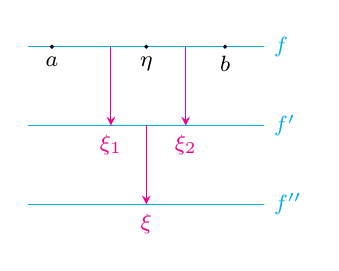
\begin{tikzpicture}[->,samples=100,>=stealth,font=\footnotesize]
            \draw [-,cyan] (0,0)--(3,0)node[right]{$f$};
            \draw [-,cyan] (0,-1)--(3,-1)node[right]{$f'$};
            \draw [-,cyan] (0,-2)--(3,-2)node[right]{$f''$};
            \draw [fill=black] (0.3,0) circle(0.5pt)node[below]{$a$};
            \draw [fill=black] (2.5,0) circle(0.5pt)node[below]{$b$};
            \draw [fill=black] (1.5,0) circle(0.5pt)node[below]{$\eta$};
            \draw [magenta] (1.05,0)--(1.05,-1)node[below]{$\xi_1$};
            \draw [magenta] (2,0)--(2,-1)node[below]{$\xi_2$};
            \draw [magenta] (1.5,-1)--(1.5,-2)node[below]{$\xi$};
        \end{tikzpicture}
        \caption{}
        \label{Lagrangexi1xi2eta}
    \end{figure}
\end{minipage}\hfill
\begin{minipage}[b]{0.3\linewidth}
    \begin{figure}[H]
        \centering
        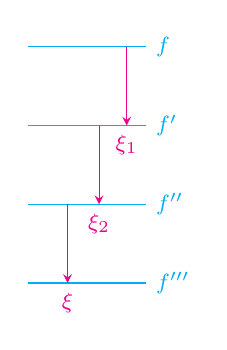
\begin{tikzpicture}[->,samples=100,>=stealth,font=\footnotesize]
            \draw [-,cyan] (0,0)--(1.5,0)node[right]{$f$};
            \draw [-,cyan] (0,-1)--(1.5,-1)node[right]{$f'$};
            \draw [-,cyan] (0,-2)--(1.5,-2)node[right]{$f''$};
            \draw [-,cyan] (0,-3)--(1.5,-3)node[right]{$f'''$};
            \draw [magenta] (1.25,0)--(1.25,-1)node[below]{$\xi_1$};
            \draw [magenta] (0.9,-1)--(0.9,-2)node[below]{$\xi_2$};
            \draw [magenta] (0.5,-2)--(0.5,-3)node[below]{$\xi$};
        \end{tikzpicture}
        \caption{}
        \label{xi1xi2xix3f}
    \end{figure}
\end{minipage}\hfill
\begin{minipage}[b]{0.3\linewidth}
    \begin{figure}[H]
        \centering
        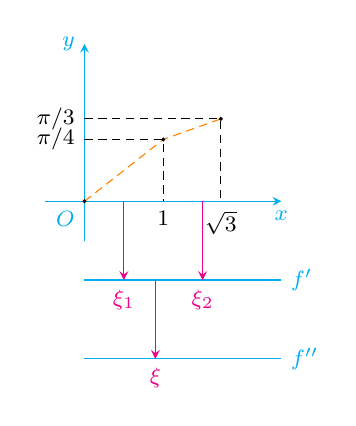
\begin{tikzpicture}[->,samples=100,>=stealth,font=\footnotesize]
            \draw[->,cyan](-0.5,0)--(0,0)node[below left]{$O$}--(2.5,0)node[below]{$x$};
            \draw[->,cyan](0,-0.5)--(0,2)node[left]{$y$};
            \draw[-,densely dashed] (0,{pi/4})node[left]{$\pi/4$}--(1,{pi/4})--(1,0)node[below]{$1$};
            \draw[-,densely dashed] (0,{pi/3})node[left]{$\pi/3$}--({sqrt(3)},{pi/3})--({sqrt(3)},0)node[below]{$\sqrt{3}$};
            \draw [-,cyan] (0,-1)--(2.5,-1)node[right]{$f'$};
            \draw [-,cyan] (0,-2)--(2.5,-2)node[right]{$f''$};
            \draw [magenta] (0.5,0)--(0.5,-1)node[below]{$\xi_1$};
            \draw [magenta] (1.5,0)--(1.5,-1)node[below]{$\xi_2$};
            \draw [magenta] (0.9,-1)--(0.9,-2)node[below]{$\xi$};
            \draw [densely dashed,orange,-] (0,0)--(1,{pi/4})--({sqrt(3)},{pi/3});
            \draw [fill=black] (0,0) circle(0.5pt);
            \draw [fill=black] (1,{pi/4}) circle(0.5pt);
            \draw [fill=black] ({sqrt(3)},{pi/3}) circle(0.5pt);
        \end{tikzpicture}
        \caption{}
        \label{pi3pi4xi1xi2}
    \end{figure}
\end{minipage}

\begin{example}
    设 $f(x)\in C[a,b]\cap D^2(a,b),~f(a)=f(b)=0,~f_+'(a)>0$,证明: $\exists\xi\in(a,b)$,使得 $f''(\xi)<0.$
\end{example}
\begin{solution}
    如图 \ref{Lagrangexi1xi2eta} 所示,因为 $f_+'(a)=\displaystyle\lim_{x\to a^+}\dfrac{f(x)-f(a)}{x-a}$,且 $f(a)=0$,因此 $\displaystyle\lim_{x\to a^+}\dfrac{f(x)}{x-a}>0$,所以 $\exists\eta\in(a,b)$,使得 $f(\eta)>0$,
    在 $[a,\eta]$ 和 $[\eta,b]$ 上分别使用 Lagrange 中值定理,有
    $$\dfrac{f(\eta)-f(a)}{\eta-a}=f'(\xi_1)>0,~\dfrac{f(b)-f(\eta)}{b-\eta}=f'(\xi_2)<0,~\xi_1\in(a,\eta),\xi_2\in(\eta,b)$$
    在 $[\xi_1,\xi_2]$ 满足 Lagrange 中值定理条件,故 $\exists\xi\in(\xi_1,\xi_2)\subset(a,b)$,使得
    $$\dfrac{f'(\xi_2)-f'(\xi_1)}{\xi_2-\xi_1}=f''(\xi)<0.$$
\end{solution}

\begin{example}
    设函数 $f(x)\in C[0,1]\cap D^3(0,1)$,且 $f(0)=f(1)=0$,又 $F(x)=x^3f(x)$,证明存在 $\xi\in(0,1)$,使得 $F'''(\xi)=0.$
\end{example}
\begin{proof}[{\songti \textbf{证法一}}]
    如图 \ref{xi1xi2xix3f} 所示,欲使在 $f'''$ 层次有一中值,则需要在 $f''$ 层次中寻找一个左右端点皆为 0 值的区间,同理 $f'$ 层次中也需要寻找两个零点,
    由已知 $F(0)=F(1)=0$ 且 $F(x)$ 在 $[0,1]$ 上可导,故由 Rolle 定理知,
    $\exists\xi_1\in(0,1)\text{,使得 }F'(\xi_1)=0$,
    又 $$F'(x)=3x^2f(x)+x^3f'(x),~F''(x)=6xf(x)+6x^2f'(x)+x^3f''(x)$$
    所以 $F'(0)=0,~F''(0)=0$,于是由 Rolle 定理知,
    $\exists\xi_2\in(0,\xi_1)\text{,使得 }F''(\xi_2)=0$,
    再由 $F''(x)$ 在 $[0,\xi_2]$ 上用 Rolle 定理知,$\exists\xi\in(0,\xi_2)\subset(0,\xi_1)\subset(0,1)\text{,使得 }F'''(\xi)=0.$
\end{proof}
\begin{proof}[{\songti \textbf{证法二}}]
    $F(x)=x^3f(x)$ 在 $[0,1]$ 上三阶可导,且 $F(0)=F(1)=0,~F'(0)=F''(0)=0$,令 $g(x)=x^3$,则 $g'(x)=3x^2>0$,$g''(x)=6x>0,~\forall x\in(0,1)$,
    由 Cauchy 中值定理知,$$\dfrac{F(1)-F(0)}{g(1)-g(0)}=\dfrac{F'(\xi_1)}{g'(\xi_1)}$$
    然后分别对 $F'(x)$ 与 $g'(x)$ 在 $[0,\xi_1]$ 和 $F''(x)$ 与 $g''(x)$ 在 $[0,\xi_2]$ 上用 Cauchy 中值定理知,
    $$0=\dfrac{F'(\xi_1)-F'(\xi_1)}{g'(\xi_1)-g'(0)}=\dfrac{F''(\xi_2)}{g''(\xi_2)}=\dfrac{F''(\xi_2)-F''(0)}{g''(\xi_2)-g''(0)}=\dfrac{F'''(\xi)}{g'''(\xi)}=\dfrac{F'''(\xi)}{6}$$
    其中 $\xi_2\in(0,\xi_1),~\xi\in(0,\xi_2)\subset(0,1)$,故得 $F'''(\xi)=0.$
\end{proof}

\begin{example}
    设函数 $\displaystyle f(x)\in C[a,b]\cap D^5(a,b)$,证明: $\exists\xi\in(a,b)$,使得
    $$f(b)=f(a)+\dfrac{1}{6}(b-a)\qty[f'(a)+f'(b)+4f'\qty(\dfrac{a+b}{2})]-\dfrac{(b-a)^5}{2880}f^{(5)}(\xi).$$
\end{example}
\begin{proof}[{\songti \textbf{证}}]
    令 $h=\dfrac{b-a}{2},~c=\dfrac{a+b}{2}$,则待证式等价为
    $$f(c+h)=f(c-h)+\dfrac{h}{3}\qty[f'(c-h)+f'(c+h)+4f'(c)]-\dfrac{h^5}{90}f^{(5)}(\xi)$$
    令 $h=x$,构造辅助函数 $$\varphi(x)=f(c+x)-f(c-x)-\dfrac{x}{3}\qty[f'(c-x)+f'(c+x)+4f'(c)]+\dfrac{x^5}{90}k$$
    即证 $k=f^{(5)}(\xi)$,因为 $f\in C[a,b]\cap D^5(a,b)$,所以 $\varphi(x)\in C[a,b]\cap D^4(a,b)$,因此
    \begin{flalign*}
        \varphi'(x)   & =\dfrac{2}{3}\qty[f'(c+x)+f'(c-x)]-\dfrac{4}{3}f'(c)+\dfrac{x}{3}\qty[f''(c-x)-f''(c+x)]+\dfrac{x^4}{18}k \\
        \varphi''(x)  & =\dfrac{1}{3}\qty[f''(c+x)-f''(c-x)]-\dfrac{x}{3}\qty[f'''(c-x)+f'''(c+x)]+\dfrac{2x^3}{9}k               \\
        \varphi'''(x) & =\dfrac{x}{3}\qty[f^{(4)}(c-x)-f^{(4)}(c+x)]+\dfrac{2x^2}{3}k
    \end{flalign*}
    因为 $\varphi(0)=\varphi(h)=0$,由 Rolle 定理知,$\exists\xi_1\in(0,h)$,使得 $\varphi'(\xi_1)=0$,而 $\varphi'(0)=0$,所以,又由 Rolle 定理知,$\exists\xi_2\in(0,\xi_1)$,使得 $\varphi''(\xi_2)=0$,最后又因为 $\varphi''(0)=0$,所以 $\exists\xi_3$,使得
    $$\varphi'''(\xi_3)=\dfrac{\xi_3}{3}\qty[f^{(4)}(c-\xi_3)-f^{(4)}(c+\xi_3)]+\dfrac{2\xi_3^2}{3}k$$
    又根据 Lagrange 中值定理,$\exists\xi_(c-\xi_3,c+\xi_3)\subset(a,b)$,使得 $$f^{(4)}(c-\xi_3)-f^{(4)}(c+\xi_3)=f^{(5)}(\xi)(-2\xi_3)$$
    即 $0=\dfrac{-2\xi_3^2}{3}f^{(5)}(\xi)+\dfrac{2\xi_3^2}{3}k\Rightarrow f^{(5)}(\xi)=k$.
\end{proof}

\subsubsection{特殊函数作差法}

\begin{example}
    设 $f(x)\in C\qty[0,\sqrt{3}]\cap D^2\qty(0,\sqrt{3})$,且 $f(0)=0,~f(1)=\dfrac{\pi}{4},~f\qty(\sqrt{3})=\dfrac{\pi}{3}$,证明: $\exists\xi\in(0,\sqrt{3})$,使得 $f''(\xi)=-\dfrac{2\xi}{1+\xi^2}f'(\xi).$
\end{example}
\begin{proof}[{\songti \textbf{证: }}]
    如图 \ref{pi3pi4xi1xi2} 所示,欲证在 $f''$ 层次有一中值,则需寻找在 $f'$ 层次的两个过渡中值,那么就需要在 $f$ 层次,即通过作差的方法将第一象限的两个坐标点,向下移动到 $x$ 轴,使得在 $x$ 轴上存在 3 个零点,
    满足这一性质的可以思考到将 $f(x)$ 与 $\arctan x$ 作差得到,即令 $g(x)=f(x)-\arctan x$,则 $g(0)=g(1)=g(\sqrt{3})=0$,由 Rolle 中值定理知 $\exists\xi_1\in(0,1),\exists_2\in(1,\sqrt{3})$,使 $g'(\xi_1)=g'(\xi_2)=0$,即
    $$\qty(1+\xi_1^2)f'(\xi_1)=\qty(1+\xi_2^2)f'(\xi_2)=1$$
    再令 $h(x)=\qty(1+x^2)f'(x)$,那么 $h(\xi_1)=h(\xi_2)$,又由 Rolle 中值定理知 $\exists\xi\in(\xi_1,\xi_2)\subset(0,\sqrt{3})$,使 $h'(\xi)=0$,整理即得待证式.
\end{proof}
% \begin{proof}[{\songti \textbf{证法二: }}]
%     由 $f(0)=0,~f(1)=\dfrac{\pi}{4},~f\qty(\sqrt{3})=\dfrac{\pi}{3}$ 构建插值多项式
%     \begin{table}[H]
%         \centering
%         \caption{}
%         \resizebox{.99\textwidth}{!}{
%             \begin{tabular}{c c c c}
%                 \toprule
%                 $x_{k}$                     & $f(x_k)$                     & 一阶差商                                                                  & 二阶差商                                                                                                   \\
%                 \midrule
%                 $x_{0}=\textcolor{cyan}{0}$ & $f_0=\textcolor{magenta}{0}$ &                                                                           &                                                                                                            \\
%                 $x_{1}=\textcolor{cyan}{1}$ & $f_1=\dfrac{\pi}{4}$         & $f[x_0,x_1]=\dfrac{f_1-f_0}{x_1-x_0}=\textcolor{magenta}{\dfrac{\pi}{4}}$ &                                                                                                            \\[6pt]
%                 $x_{2}=\sqrt{3}$            & $f_2=\dfrac{\pi}{3}$         & $f[x_1,x_2]=\dfrac{f_2-f_1}{x_2-x_1}=\dfrac{\pi}{12\qty(\sqrt{3}-1)}$     & $f[x_0,x_1,x_2]=\dfrac{f[x_1,x_2]-f[x_0,x_1]}{x_2-x_0}=\textcolor{magenta}{\dfrac{3\pi-5\sqrt{3}\pi}{72}}$ \\
%                 \bottomrule
%             \end{tabular}}
%     \end{table}
%     则插值多项式为 
%     $$p(x)=\textcolor{magenta}{0}+\textcolor{magenta}{\dfrac{\pi}{4}}(x-\textcolor{cyan}{0})+\textcolor{magenta}{\dfrac{3\pi-5\sqrt{3}}{72}}(x-\textcolor{cyan}{0})(x-\textcolor{cyan}{1})=\dfrac{\pi}{4}x+\dfrac{3\pi-5\sqrt{3}\pi}{72}x(x-1)$$
%     因此令 $F(x)=f(x)-p(x)$,则 $F(0)=F(1)=F\qty(\sqrt{3})=0$
% \end{proof}

\subsubsection{合理分配法}

\begin{example}
    设 $f(x)\in C\qty[-\dfrac{\pi}{2},\dfrac{\pi}{2}]\cap D\qty(-\dfrac{\pi}{2},\dfrac{\pi}{2}),~f(0)=0$,
    证明: $\exists\xi\in\qty(-\dfrac{\pi}{2},\dfrac{\pi}{2})$,使得 $$f''(\xi)=3f'(\xi)\tan\xi+2f(\xi).$$
\end{example}
\begin{proof}[{\songti \textbf{证}}]
    构造辅助函数\footnote{
        首先观察待证式的各项系数,发现存在 $1+2=3$ 的情况,于是利用“合理分配达到平均”思想,组成 $$f''(\xi)-f'(\xi)\tan\xi=2\qty[f'(\xi)\tan\xi+f(\xi)]$$
        又 $\cos\xi\neq0$,于是两边同时乘以 $\cos\xi$,得 $\qty[f''(\xi)\cos\xi-f'(\xi)\sin\xi]-2\qty[f'(\xi)\sin\xi+f(\xi)\cos\xi]=0$;
        发现 $[]$ 内是“前导后不导”形式,则可化为 $g'(\xi)=\qty(f'(\xi)\cos\xi)'-2\qty(f(\xi)\sin\xi)'=0$,$g(x)=f'(x)\cos x-2f(x)\sin x$;
        此为“经典构造模型”之一 (参考表 \ref{fuzuhansgzao}),则构造辅助函数 $$F(x)=f(x)\e^{\int-2\tan x\dd x}=f(x)\cdot\cos^2x.$$
    } $F(x)=f(x)\cdot\cos^2x$,那么有 $F\qty(-\dfrac{\pi}{2})=F\qty(\dfrac{\pi}{2})=F(0)=0$,则由 Rolle 定理知,
    $\exists\xi_1,\xi_2$ 分别属于 $\qty(-\dfrac{\pi}{2},0)$ 与 $\qty(0,\dfrac{\pi}{2})$,使得 $F'(\xi_1)=F'(\xi_2)=0$,又
    $$F'(x)=f'(x)\cos^2x-2\sin x\cos xf(x)=\cos x\qty[f'(x)\cos x-2\sin xf(x)]$$
    令 $g(x)=f'(x)\cos x-2\sin xf(x)$,则有 $g(\xi_1)=g(\xi_2)=0$,再由 Rolle 定理知,
    $\exists\xi\in(\xi_1,\xi_2)\subset\qty(-\dfrac{\pi}{2},\dfrac{\pi}{2})$,使得
    $$g'(\xi)=0=f''(\xi)\cos \xi-3f(\xi)\sin\xi-2f(\xi)\cos\xi$$
    由于 $\cos\xi\neq0$,所以两边同时除以 $\cos\xi$,即得证.
\end{proof}

\subsubsection{补充导函数法}

一般待证式中,出现的导函数阶数是连续的,即 0 与 1 或 1 与 2,亦或常数与导函数直接相等的类型,当缺失一阶导函数的时候,需要人为补充一阶导,之后再构造辅助函数.

\begin{example}
    设函数 $f(x)\in C[a,b]\cap D^2(a,b)$,且 $f(a)=f'(a)=f''(a)=f(b)=0$,证明: $\exists \xi\in(a,b)$,使得 $(\xi-a)^2f''(\xi)-2f(\xi)=0.$
\end{example}
\begin{proof}[{\songti \textbf{证}}]
    先令\footnote{因为缺少一阶导项,故考虑人为补充,又由待证式的结构不难想到 $\qty(gf'-fg')'$ 其中 $g=(x-a)^2$.} $F(x)=(x-a)^2f'(x)-2f(x)(x-a)$,则 $F(a)=0$,欲再寻找一点 $\eta$,使得 $F(\eta)=0$,为此构造辅助函数
    $$G(x)=\begin{cases}
            \dfrac{f(x)}{(x-a)^2}, & x\in(a,b] \\
            0,                     & x=a
        \end{cases}$$
    则有 $\displaystyle\lim_{x\to a^+}G(x)=\lim_{x\to a^+}\dfrac{f(x)}{(x-a)^2} =\lim_{x\to a^+}\dfrac{f(a)+f'(a)(x-a)+\dfrac{1}{2!}f''(a)(x-a)^2+o\qty((x-a)^2)}{(x-a)^2}=0=G(0)$,
    因此 $G(x)$ 在 $[a,b]$ 上连续,在 $(a,b)$ 内可导,且 $G(a)=G(b)$ 则由 Rolle 定理知
    $\exists\eta\in(a,b)$,使得 $$G'(\eta)=\dfrac{f'(\eta)(\eta-a)^2-2(\eta-a)f(\eta)}{(\eta-a)^4}=0\Rightarrow f'(\eta)(\eta-a)^2-2(\eta-a)f(\eta)=0\Rightarrow F(\eta)=0$$
    又因为 $F(x)$ 在 $[a,b]$ 上连续,$(a,b)$ 内可导,故由 Rolle 定理知 $\exists\xi\in(a,b)$,使得 $$F'(\xi)=2(\xi-a)f'(\xi)+(\xi-a)^2f''(\xi)-2f'(\xi)(\xi-a)-2f(\xi)=0$$
    整理即得证 $(\xi-a)^2f''(\xi)-2f(\xi)=0.$
\end{proof}
